\chapter{Implementaci\'on de la Solución.}

\section{Arquitectura final de la solución}

Finalmente, se optó por utilizar el framework MVC Ruby on Rails para el desarrollo de la aplicación web, conocida por su robustez y facilidad de uso.
Para la base de datos, se optó por Neo4j, ya que posee una gran comunidad y es la que recibe más soporte, de las opciones posibles. 

%falta explicar mas la arqui

\section{Caso de ejemplo}

Cuando un usuario ingresa al sistema, lo primero que se ve es la sección de ítems recomendados, 

\begin{figure}[hbtp]
\centering

\includegraphics[scale=0.7]{images/screen2.png}
\caption{La sección de items recomendados para el usuario, ordenados según el puntaje predicho.}
\end{figure} 

El ítem de mayor tamaño es el que obtuvo la mayor calificación predicha. Cuando el usuario selecciona ese lugar, se ve la siguiente pantalla.

\begin{figure}[hbtp]
\centering

\includegraphics[scale=0.7]{images/screen1.png}
\caption{La vista del Centro Cultural GAM, donde se puede ver una breve descripción del lugar, junto con lsa opiniones de usuarios que visitaron el lugar.}
\end{figure}  




A continuación se detallará el proceso de implementación del sistema. Junto con un ejemplo detallado de la evolución de las variables involucradas y la forma en que se llega a el resultado final, la lista de ítems recomendados al usuario.

Para facilitar la comprensión del funcionamiento del algoritmo, se va a usar el siguiente ejemplo:

\begin{figure}
\centering
\begin{adjustbox}{max width=\textwidth}
\begin{tabular}{l*{6}{c}r}
                  & Plaza de Armas & Cerro Sta. Lucia & Cerro San Cristobal & Museo de Bellas Artes & Quinta Normal  & Teatro Municipal & Centro GAM \\
\hline
Juan          & 5 & 4 & 2 &   & 1 &   &   \\
\hline
Ignacio       & 3 &   & 2 &   & 5 &   & 4 \\
\hline
Perla         & 3 & 3 &   & 1 & 4 & 3 &   \\
\hline
Inés          & 5 & 5 &   & 1 & 2 &   & 5 \\
\hline
Sam          & 1 &  &   &  &  & 4  & 3 \\


\end{tabular}
\end{adjustbox}
\caption{Las estrellas que dan los usuarios A, B, C y D a distintas películas} 

\end{figure}

\begin{figure}[hbtp]
\centering
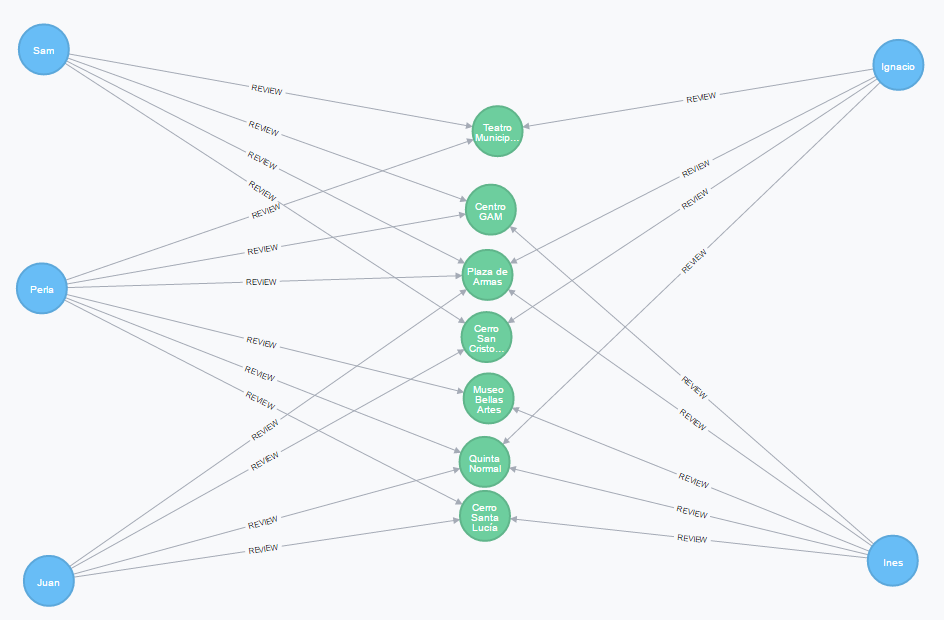
\includegraphics[scale=0.8]{images/examplegraph.png}
\caption{El grafo que se produce al relacionar la reseñas de los usuarios del sistema y los lugares disponibles para visitar}
\end{figure}  

En este ejemplo, el usuario que entra al sistema y cuyos puntajes son predichos se conoce como consumidor, en este caso es el Usuario 1.

Cada ítem para el cual el consumidor aún no ha escrito una review y que se encuentre a cierta distancia geográfica es un potencial ítem recomendado, pero antes es necesario conocer qué puntaje le asignaría el consumidor.

\begin{figure}
\centering
\begin{adjustbox}{max width=\textwidth}
\begin{tabular}{l*{6}{c}r}
                  & Plaza de Armas & Cerro Sta. Lucia & Cerro San Cristobal & Museo de Bellas Artes & Quinta Normal  & Teatro Municipal & Centro GAM \\
\hline
\rowcolor{yellow} Juan          & 5 & 4 & 2 &   & 1 &   &   \\
\hline
Ignacio       & 3 &   & 2 &   & 5 &   & 4 \\
\hline
\rowcolor{yellow}Perla         & 3 & 3 &   & 1 & 4 & 3 &   \\
\hline
\rowcolor{yellow}Inés          & 5 & 5 &   & 1 & 2 &   & 5 \\
Sam          & 1 &  &   &  &  & 4  & 3 \\


\end{tabular}
\end{adjustbox}
\caption{La misma tabla de la figura x, imaginar que se quiere conocer el puntaje que Juan dará al Museo de Bellas Artes, para eso se deben tener en cuenta sólo los usuarios que hayan visitado este lugar, o sea, Perla y Inés.}

\end{figure}

Comenzando por el primer ítem candidato, al iniciar la sesión, el sistema consulta por todas las reviews que hayan sido escritas sobre el ítem actual. Los usuarios que escribieron estas reviews se conocen como productores.

De este grupo de productores, se escogen sólo los que hayan escrito reseñas sobre al menos dos ítems sobre los que el consumidor haya también dado su opinión.
\newcolumntype{g}{>{\columncolor{yellow}}c}
\begin{figure}
\centering
\begin{adjustbox}{max width=\textwidth}
\begin{tabular}{|c|g|g|c|c|g|c|c|}

                  & Plaza de Armas & Cerro Sta. Lucia & Cerro San Cristobal & Museo de Bellas Artes & Quinta Normal  & Teatro Municipal & Centro GAM \\
\hline
Juan          & 5 & 4 & 2 &   & 1 &   &   \\
\hline
\rowcolor{white}Ignacio       & 3 &   & 2 &   & 5 &   & 4 \\
\hline
Perla         & 3 & 3 &   & 1 & 4 & 3 &   \\
\hline
Inés          & 5 & 5 &   & 1 & 2 &   & 5 \\
\hline
Sam          & 1 &  &   &  &  & 4  & 3 \\
\hline

\end{tabular}
\end{adjustbox}
\caption{Tabla x, pero destacando que para el cálculo del puntaje al Museo de Bellas artes, sólo se tomaran en cuenta lugares que hayan sido visitados por los tres usuarios, Juan, Perla e Inés.}

\end{figure}


En la sección de estado del arte se describieron varias formas en que se pueden integrar los algoritmos de recomendación con los de trust. Para este dominio en particular, ya que se intenta hacer un acercamiento al comportamiento observado en la vida diaria entre personas, se decidió que se utilizará el trust como un umbral, en el que la opinión de una persona ''no confiable'' se considera inválida y por lo tanto, es ignorada. 

Por lo tanto, después de determinar los posibles usuarios productores, existe otro filtro que determina quiénes serán de confianza. Después de obtener la lista inicial de productores, se determina el nivel de trust que tiene el consumidor con cada uno de los productores. Si no existe una relación directa de trust entre el consumidor y el posible productor, ésta se calcula mediante ''tidal trust''. Una vez que se tiene el valor de trust, el productor candidato es removido de la lista si es que su trust con el consumidor es menor a 0.5, en caso contrario, permanece en la lista. 

Luego, para estimar numéricamente el parecido de las opiniones del consumidor con cada productor, se utiliza la correlación de Pearsson (cita). La idea detrás de esta lógica es que mientras más parecido sea el consumidor con un productor, más peso tendrá éste sobre la estimación del puntaje predicho. Empezando por Juan y Perla:

\begin{figure}

\begin{equation}
sim(u,n)=\frac{\sum_{i=1}^{n}(u_i-\bar{u})(n_i-\bar{n})}{\sqrt{\sum_{i=1}^{n}(u_i-\bar{u})^2}+\sqrt{\sum_{i=1}^{n}(n_i-\bar{n})^2}}
\end{equation}
\caption{La similitud entre dos conjuntos, según la correlación de Pearsson, en este caso, interpretar los valores de $u$ como las estrellas que ha dado Juan a los lugares que visitó y los de $n$ los que ha dado Perla. }

\end{figure}
Conociendo el puntaje que ha puesto en promedio cada productor, $\bar{u}$ para Juan y $\bar{n}$ para Perla, se calcula la diferencia con el puntaje dado. Reemplazando con los promedios y los valores de reseñas, se tiene:


\begin{equation}
\frac{3*-1.5 + 2*3.5+-1*-0.5}{\sqrt{3^2+2^2+(-1)^2}*\sqrt{(-0.5)^2+(-1.5)^2+(-1,5)^2+o.5^2+3,5^2+(-0.5)^2}}  = 0.3785
\end{equation}


Este proceso se repite para cada dupla de consumidor-productor posible.

Con esto, se tiene el numerador de la ecuación (referencia), el denominador es el producto de las sumatorias de las desviaciones estándares, para Juan y para Perla.

Con esto, se llega finalmente a un puntaje estimado, que dará el consumidor al ítem actual. Este proceso se repite para cada ítem candidato.
Luego, cuando ya se tienen todos los puntajes predichos, se considera como recomendables sólo los ítems cuyo puntaje estimado sea al menos 3 estrellas.


\begin{figure}
\centering
\begin{adjustbox}{max width=\textwidth}
\begin{tabular}{|c|c|c|c|}
\hline
                &   Museo de Bellas Artes & Teatro Municipal & Centro GAM \\

\hline
Puntaje Predicho Juan          & 1.28  &  3.60  & 3.09  \\
\hline


\end{tabular}
\end{adjustbox}
\caption{Se pueden ver los puntajes que el sistema predice para Juan, se puede ver que el sistema estima que a Juan no le va a gustar el Museo de Bellas Artes, sin embargo, se puede ver que dará puntajes por sobre 3 estrellas al Teatro Municipal y al Centro GAM, por lo tanto se les recomienda esos lugares a Juan.}

\end{figure}

% otra vista que muestra la pantalla de recomendación

Son estos los ítems que el sistema va a mostrar en la vista de recomendados, ordenados de mayor a menor puntaje. 
